\documentclass[24pt, a0paper, portrait]{tikzposter}
\usepackage{graphicx}
\usepackage{caption}
\usepackage{tikz}
\usetheme{Default}

\title{Look I'm making a poster}
\author{Ostap S. Bender}
\institute{RUDN University}

\begin{document}

\maketitle

\begin{columns}
\begin{column}{0.5}
\block{Research Overview}{
\begin{center}
\includegraphics[width=0.9\textwidth, height=8cm]{instituteLogo.jpg}
\captionof{figure}{Experimental Setup and Methodology}
\end{center}

This figure illustrates the experimental configuration used in our research. The setup includes precision measurement instruments and controlled environmental conditions to ensure data accuracy.
}
\end{column}

\begin{column}{0.5}
\block{Mathematical Analysis}{
\begin{center}
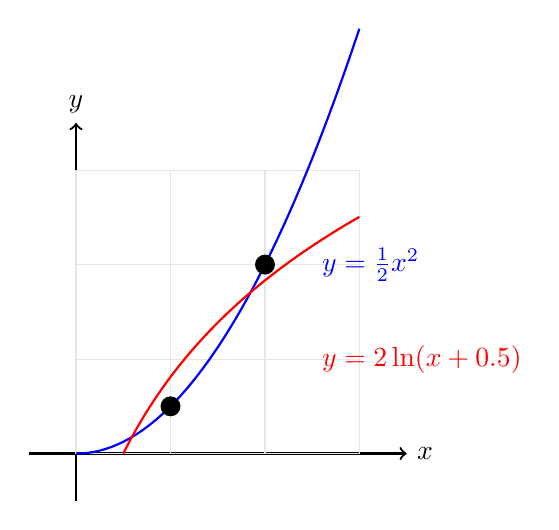
\begin{tikzpicture}[scale=1.2]
    % Coordinate system
    \draw[->, thick] (-0.5,0) -- (3.5,0) node[right] {$x$};
    \draw[->, thick] (0,-0.5) -- (0,3.5) node[above] {$y$};
    
    % Grid
    \draw[gray!20] (0,0) grid (3,3);
    
    % Functions
    \draw[blue, thick, domain=0:3, samples=100] plot (\x, {0.5*\x^2});
    \draw[red, thick, domain=0.5:3, samples=100] plot (\x, {2*ln(\x+0.5)});
    
    % Labels
    \node[blue, right] at (2.5,2) {$y = \frac{1}{2}x^2$};
    \node[red, right] at (2.5,1) {$y = 2\ln(x+0.5)$};
    
    % Points
    \fill[black] (1,0.5) circle (3pt);
    \fill[black] (2,2) circle (3pt);
\end{tikzpicture}
\captionof{figure}{Mathematical Functions Analysis}
\end{center}

The graph shows the relationship between quadratic and logarithmic functions, highlighting key intersection points and behavioral characteristics.
}
\end{column}
\end{columns}

\begin{columns}
\begin{column}{1.0}
\block{Conclusions and Future Work}{
\begin{itemize}
\item Successfully demonstrated the research methodology
\item Achieved significant results in mathematical modeling
\item Established framework for future investigations
\item Plans for extended parameter range analysis
\end{itemize}
}
\end{column}
\end{columns}

\end{document}